\chapter{Evalutation}
\label{ch:Evalutation}
The optimal configuration for the different algorithms has been worked out in chapter \ref{ch:Algorithm configuration}. Now this chapter is devoted to comparing and deciding on an optimal algorithm for the problem of collision detection.\\
To be able to compare the algorithms they are each used to train a model with the hyper-parameters found in chapter \ref{ch:Analysis of the pattern recognition problem}. The models are evaluated with a k-fold validation, with k=10. The results can be seen in figure \ref{fig:ranking}.


\begin{figure}[h]
\centering
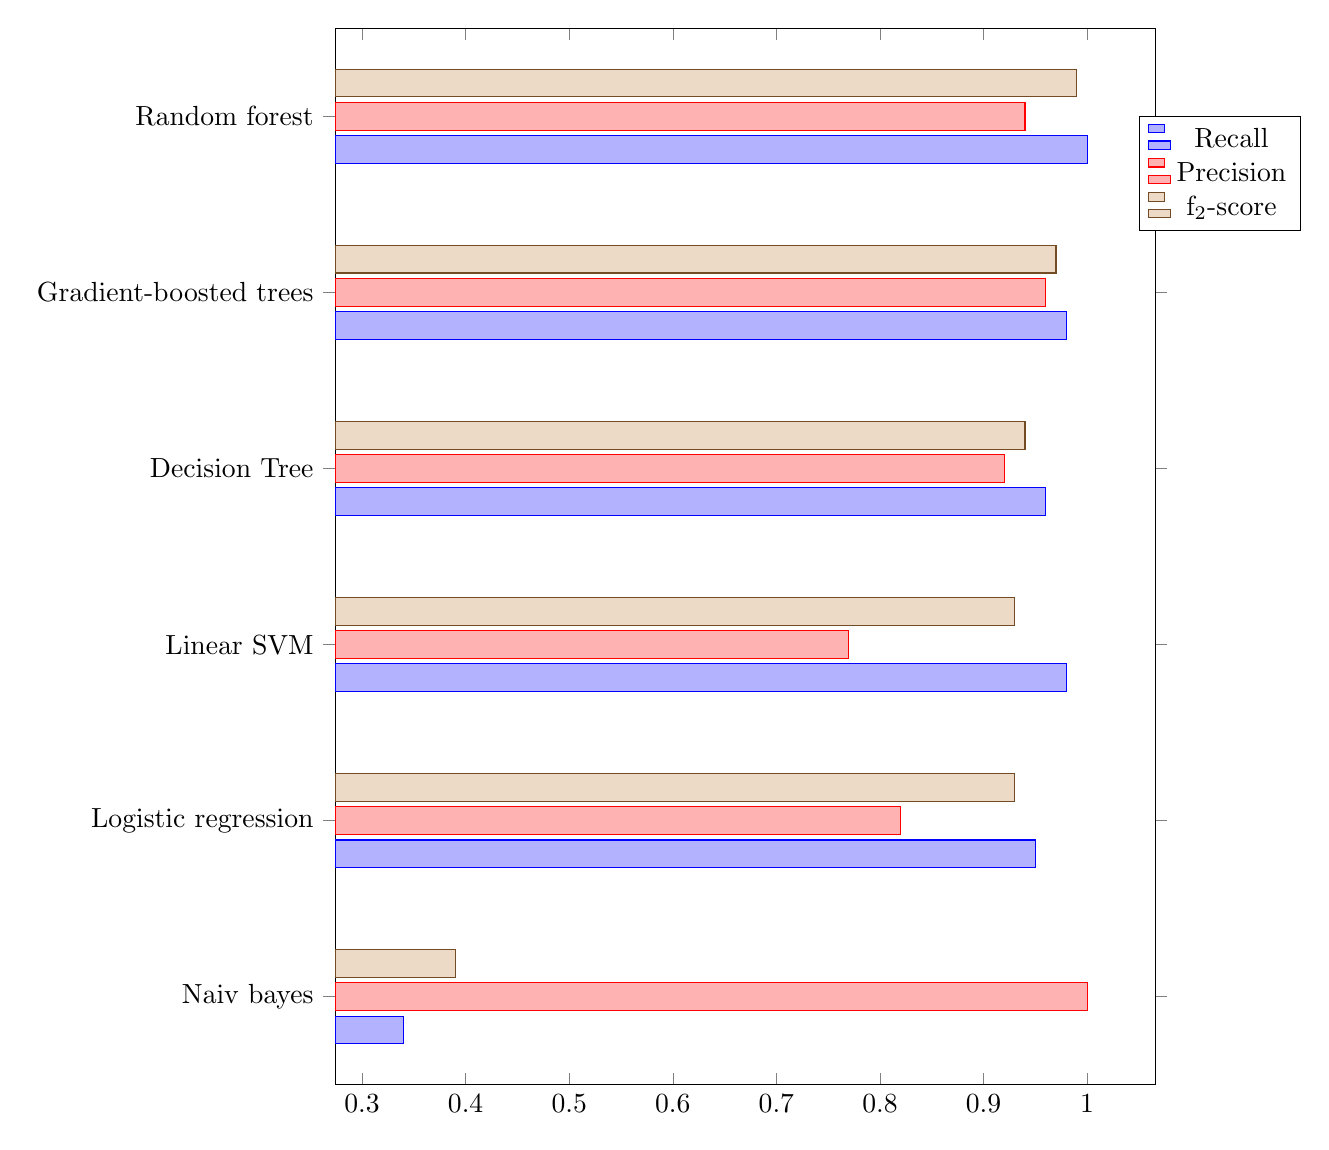
\begin{tikzpicture}
\begin{axis}[
xbar,
enlarge y limits=0.5,
%xlabel={f\textsubscript{2}-score},
width=12cm, height=15cm, enlarge y limits=0.1,
symbolic y coords={
Naiv bayes,
Logistic regression,
Linear SVM,
Decision Tree,
Gradient-boosted trees,
Random forest
},
ytick=data,
legend style={at={(axis cs:1.05,Random forest)},anchor=north west}
]

\addplot coordinates {
(1.00,Random forest)
(0.98,Linear SVM)
(0.95,Logistic regression)
(0.96,Decision Tree)
(0.98,Gradient-boosted trees)
(0.34,Naiv bayes)
};
\addplot coordinates {
(0.94,Random forest)
(0.77,Linear SVM)
(0.82,Logistic regression)
(0.92,Decision Tree)
(0.96,Gradient-boosted trees)
( 1.00,Naiv bayes)
};
\addplot coordinates {
(0.99,Random forest)
(0.93,Linear SVM)
(0.93,Logistic regression)
(0.94,Decision Tree)
(0.97,Gradient-boosted trees)
(0.39,Naiv bayes)
};

\legend{Recall, Precision, f\textsubscript{2}-score}
\end{axis}
\end{tikzpicture}

\caption{Ranking of classification algorithms}
\label{fig:ranking}
\end{figure}

According to the  f\textsubscript{2}-score the best performing method is a random forest classifier with 4 equally well performing hyper-parameter configurations:\\

Number of trees: \textbf{4}  \qquad 
Impurity:  \textbf{Entropy}  \qquad 
Maximal depth: \ \textbf{2}  \qquad 
\\
Number of trees: \textbf{4}  \qquad 
Impurity:  \textbf{Entropy}  \qquad 
Maximal depth: \ \textbf{3}  \qquad
\\
Number of trees: \textbf{9}  \qquad 
Impurity:  \textbf{Entropy}  \qquad 
Maximal depth: \ \textbf{2}  \qquad
\\
Number of trees: \textbf{10}  \qquad 
Impurity:  \textbf{Entropy}  \qquad 
Maximal depth: \ \textbf{2}  \qquad
\\ 


The best performing random forest model reaches a maximal {f\textsubscript{2}-score of \textbf{0.99} (precision:  0.94, recall: 1.0).
\\
This means a collisions that occur will be classified correctly classified as a collision 100\% of the time on the collected data and will be falsely classified as a collision 6\% of the time when no actual collision happened.
\\
This results indicate that the machine learning approach to recognizing collisions on a physical board is eligible and can perform well. Still it has to be considered that these results are achieved on data which is generated in experience soly for that reason and results may differ when applied in real world situations.
\\
In figure \ref{fig:ranking} the ranking of the classification methods shows that decision tree based approaches have a advantage over the remaining algorithms. Random forest and gradient-boosted tree models as decision tree assembles performed on average better than a single decision tree. The naiv base algorithm performs worst under the possible algorithms. 
